% Arquivo LaTeX de exemplo de dissertação/tese a ser apresentada à CPG do IME-USP
%
% Criação: Jesús P. Mena-Chalco
% Revisão: Fabio Kon e Paulo Feofiloff
% Adaptação para UTF8, biblatex e outras melhorias: Nelson Lago
%
% Except where otherwise indicated, these files are distributed under
% the MIT Licence. The example text, which includes the tutorial and
% examples as well as the explanatory comments in the source, are
% available under the Creative Commons Attribution International
% Licence, v4.0 (CC-BY 4.0) - https://creativecommons.org/licenses/by/4.0/


%%%%%%%%%%%%%%%%%%%%%%%%%%%%%%%%%%%%%%%%%%%%%%%%%%%%%%%%%%%%%%%%%%%%%%%%%%%%%%%%
%%%%%%%%%%%%%%%%%%%%%%%%%%%%%%% PREÂMBULO LaTeX %%%%%%%%%%%%%%%%%%%%%%%%%%%%%%%%
%%%%%%%%%%%%%%%%%%%%%%%%%%%%%%%%%%%%%%%%%%%%%%%%%%%%%%%%%%%%%%%%%%%%%%%%%%%%%%%%

% A opção twoside (frente-e-verso) significa que a aparência das páginas pares
% e ímpares pode ser diferente. Por exemplo, as margens podem ser diferentes ou
% os números de página podem aparecer à direita ou à esquerda alternadamente.
% Mas nada impede que você crie um documento "só frente" e, ao imprimir, faça
% a impressão frente-e-verso.
%
% Aqui também definimos a língua padrão do documento (a última da lista) e
% línguas adicionais. Para teses do IME, no mínimo português e inglês são
% obrigatórios, porque independentemente da língua principal do texto é
% preciso fornecer o resumo nessas duas línguas. LaTeX aceita alguns nomes
% diferentes para a língua portuguesa; dentre as opções, prefira sempre
% "brazilian" para português brasileiro e "portuguese" para português europeu.
%\documentclass[a4paper,12pt,twoside,brazilian,english]{book}
\documentclass[a4paper,12pt,twoside,english,brazilian]{book}

% O preâmbulo de um documento LaTeX pode ser razoavelmente longo. Neste
% modelo, optamos por reduzi-lo, colocando praticamente tudo do preâmbulo
% nas packages "imegoodies" e "imelooks".
%
% imegoodies carrega diversas packages muito úteis e populares (algumas
% são praticamente obrigatórias, como amsmath, babel, array etc.). É
% uma boa ideia usá-la com outros documentos também. Ela inclui vários
% comentários explicativos e dicas de uso; não tenha medo de alterá-la
% conforme a necessidade.
%
% imelooks carrega algumas packages e configurações que definem a
% aparência do documento; você também pode querer usá-la (ou partes
% dela) com outros documentos para obter as mesmas fontes, margens
% etc. Tal como "imegoodies", pode valer a pena ler os comentários
% e fazer modificações nessa package. Com a opção "thesis", imelooks
% também define os comandos para capa, folha de rosto etc.
\usepackage{imegoodies}
\usepackage[thesis]{imelooks}

%\nocolorlinks % para impressão em P&B


% Diretórios onde estão as figuras; com isso, não é necessário (mas
% é permitido) colocar o caminho completo em \includegraphics. Note
% que a extensão nunca é necessária (mas é permitida), ou seja, o
% resultado é o mesmo com "\includegraphics{figuras/foto.jpeg}",
% "\includegraphics{foto.jpeg}", "\includegraphics{figuras/foto}"
% ou "\includegraphics{foto}".
\graphicspath{{figuras/},{fig/},{logos/},{img/},{images/},{imagens/}}

% Comandos rápidos para mudar de língua:
% \en -> muda para o inglês
% \br -> muda para o português
% \texten{blah} -> o texto "blah" é em inglês
% \textbr{blah} -> o texto "blah" é em português
\babeltags{br = brazilian, en = english}

% O arquivo com os dados bibliográficos para biblatex; você pode usar
% este comando mais de uma vez para acrescentar múltiplos arquivos
\addbibresource{bibliografia.bib}

% Este comando permite acrescentar itens à lista de referências sem incluir
% uma referência de fato no texto (pode ser usado em qualquer lugar do texto)
%\nocite{bronevetsky02,schmidt03:MSc, FSF:GNU-GPL, CORBA:spec, MenaChalco08}
% Com este comando, todos os itens do arquivo .bib são incluídos na lista
% de referências
%\nocite{*}

% É possível definir como determinadas palavras podem (ou não) ser
% hifenizadas; no entanto, a hifenização automática geralmente funciona bem
\babelhyphenation{documentclass latexmk soft-ware clsguide} % todas as línguas
\babelhyphenation[brazilian]{Fu-la-no}
\babelhyphenation[english]{what-ever}

% Estes comandos definem o título e autoria do trabalho e devem sempre ser
% definidos, pois além de serem utilizados para criar a capa, também são
% armazenados nos metadados do PDF. O subtítulo é opcional.
\title{Florestas geradoras maximais de custo mínimo em grafos dinâmicos}[]
\translatedtitle{Title of the document}[a subtitle]

\author[fem]{Chung Jin Shian}

\def\profa{Prof\kern.02em.\kern-.07emª\kern.07em}
\def\dra{Dr\kern-.04em.\kern-.11emª\kern.07em}

% Para TCCs, este comando define o supervisor
\orientador[fem]{\profa{} \dra{} Cristina Gomes Fernandes}

\banca{
  \profa{} \dra{} Cristina Gomes Fernandes (orientadora) -- IME-USP [sem ponto final],
  % Em inglês, não há o "ª"
  %Prof. Dr. Fulana de Tal (advisor) -- IME-USP [sem ponto final],
  Prof. Dr. Ciclano de Tal -- IME-USP [sem ponto final],
  \profa{} \dra{} Convidada de Tal -- IMPA [sem ponto final],
  }
  
  % A página de rosto da versão para depósito (ou seja, a versão final
% antes da defesa) deve ser diferente da página de rosto da versão
% definitiva (ou seja, a versão final após a incorporação das sugestões
% da banca).
\tipotese{
  %mestrado,
  %doutorado,
  tcc,
  %definitiva, % É a versão para defesa ou a versão definitiva?
  %quali, % É qualificação?
  programa={Ciência da Computação},
  }
  
  \defesa{
  local={São Paulo},
  data=2025-06-02, % YYYY-MM-DD
  }
  
  \direitos{CC-BY}
  
  % Para gerar a ficha catalográfica, acesse https://fc.ime.usp.br/,
% preencha o formulário e escolha a opção "Gerar Código LaTeX".
% Basta copiar e colar o resultado aqui.
\fichacatalografica{}


%%%%%%%%%%%%%%%%%%%%%%%%%%%%%%%%%%%%%%%%%%%%%%%%%%%%%%%%%%%%%%%%%%%%%%%%%%%%%%%%
%%%%%%%%%%%%%%%%%%%%%%% AQUI COMEÇA O CONTEÚDO DE FATO %%%%%%%%%%%%%%%%%%%%%%%%%
%%%%%%%%%%%%%%%%%%%%%%%%%%%%%%%%%%%%%%%%%%%%%%%%%%%%%%%%%%%%%%%%%%%%%%%%%%%%%%%%

\usepackage{float}       % for [H]
\usepackage{subcaption}  
\newcommand{\dotvar}[2]{#1.\textit{#2}}
\newcommand{\dotvarm}[3]{\ensuremath{#1.\,\textit{#2}\!\left[#3\right]}}

\begin{document}

%%%%%%%%%%%%%%%%%%%%%%%%%%% CAPA E PÁGINAS INICIAIS %%%%%%%%%%%%%%%%%%%%%%%%%%%%

% Aqui começa o conteúdo inicial que aparece antes do capítulo 1, ou seja,
% página de rosto, resumo, sumário etc. O comando frontmatter faz números
% de página aparecem em algarismos romanos ao invés de arábicos e
% desabilita a contagem de capítulos.
\frontmatter

\pagestyle{plain}

\onehalfspacing % Espaçamento 1,5 na capa e páginas iniciais

\maketitle % capa e folha de rosto

%%%%%%%%%%%%%%%% DEDICATÓRIA, AGRADECIMENTOS, RESUMO/ABSTRACT %%%%%%%%%%%%%%%%%%



% Reinicia o contador de páginas (a próxima página recebe o número "i") para
% que a página da dedicatória não seja contada.

% Agradecimentos:
% Se o candidato não quer fazer agradecimentos, deve simplesmente eliminar
% esta página. A epígrafe, obviamente, é opcional; é possível colocar
% epígrafes em todos os capítulos. O comando "\chapter*" faz esta seção
% não ser incluída no sumário.
\chapter*{Agradecimentos}
\epigrafe{It is perhaps a more fortunate destiny to have a taste for collecting shells than to be born a millionaire}{Robert Louis Stevenson}

Primeiramente gostaria de agradecer ao...

%!TeX root=../tese.tex
%("dica" para o editor de texto: este arquivo é parte de um documento maior)
% para saber mais: https://tex.stackexchange.com/q/78101

% As palavras-chave são obrigatórias, em português e em inglês, e devem ser
% definidas antes do resumo/abstract. Acrescente quantas forem necessárias.
\palavraschave{grafo dinâmico, floresta geradora maximal de custo mínimo, splay trees}

\keywords{dynamic graph, minimum spanning forest, splay trees}

% O resumo é obrigatório, em português e inglês. Estes comandos também
% geram automaticamente a referência para o próprio documento, conforme
% as normas sugeridas da USP.
\resumo{
Grafos dinâmicos permitem modelar problemas em
que o conjunto de arestas do grafo sofre alterações
ao longo do tempo. Um dos problemas fundamentais nesse contexto é a manutenção de uma árvore geradora de custo mínimo do grafo dinâmico no decorrer de várias alterações no grafo. Neste trabalho, estudamos e implementamos vários algoritmos propostos por Holm, de Lichtenberg e Thorup~\cite{jacob_holm} para variantes desse problema. O foco foi no algoritmo para manter uma
floresta geradora maximal de custo mínimo (MSF) decremental, que dá suporte eficiente à remoção de arestas. Além disso, estudamos e apresentamos a ideia  do problema de manter uma floresta geradora maximal de custo mínimo (MSF) dinâmica, que dá suporte eficiente à adição e remoção de arestas.}

\abstract{
Dynamic graphs allow us to model problems in which the set of edges changes over time. One of the fundamental problems in this context is maintaining a minimum spanning tree of the dynamic graph as it undergoes multiple updates. In this work, we study and implement several algorithms proposed by Holm, de Lichtenberg, and Thorup~\cite{jacob_holm} for variants of this problem. Our main focus is the algorithm for maintaining a decremental minimum spanning forest, which efficiently supports edge deletions. In addition, we study and outline the approach for maintaining a fully dynamic minimum spanning forest, which efficiently supports both edge insertions and deletions.
}


%%%%%%%%%%%%%%%%%%%%%%%%%%% LISTAS DE FIGURAS ETC. %%%%%%%%%%%%%%%%%%%%%%%%%%%%%

% Como as listas que se seguem podem não incluir uma quebra de página
% obrigatória, inserimos uma quebra manualmente aqui.
\cleardoublepage

% Todas as listas são opcionais; Usando "\chapter*" elas não são incluídas
% no sumário. As listas geradas automaticamente também não são incluídas por
% conta das opções "notlot" e "notlof" que usamos para a package tocbibind.

% Normalmente, "\chapter*" faz o novo capítulo iniciar em uma nova página, e as
% listas geradas automaticamente também por padrão ficam em páginas separadas.
% Como cada uma destas listas é muito curta, não faz muito sentido fazer isso
% aqui, então usamos este comando para desabilitar essas quebras de página.
% Se você preferir, comente as linhas com esse comando e des-comente as linhas
% sem ele para criar as listas em páginas separadas. Observe que você também
% pode inserir quebras de página manualmente (com \clearpage, veja o exemplo
% mais abaixo).
\newcommand\disablenewpage[1]{{\let\clearpage\par\let\cleardoublepage\par #1}}

\newcommand{\Oh}{\mathrm{O}}

% Nestas listas, é melhor usar "raggedbottom" (veja basics.tex). Colocamos
% a opção correspondente e as listas dentro de um grupo para ativar
% raggedbottom apenas temporariamente.
\bgroup
\raggedbottom

%%%%% Listas criadas manualmente

% Quebra de página manual

%%%%% Listas criadas automaticamente


% Sumário (obrigatório)
\tableofcontents

\egroup % Final de "raggedbottom"

% Referências indiretas ("x", veja "y") para o índice remissivo (opcionais,
% pois o índice é opcional). É comum colocar esses itens no final do documento,
% junto com o comando \printindex, mas em alguns casos isso torna necessário
% executar texindy (ou makeindex) mais de uma vez, então colocar aqui é melhor.
\index{Inglês|see{Língua estrangeira}}
\index{Figuras|see{Floats}}
\index{Tabelas|see{Floats}}
\index{Código-fonte|see{Floats}}
\index{Subcaptions|see{Subfiguras}}
\index{Sublegendas|see{Subfiguras}}
\index{Equações|see{Modo matemático}}
\index{Fórmulas|see{Modo matemático}}
\index{Rodapé, notas|see{Notas de rodapé}}
\index{Captions|see{Legendas}}
\index{Versão original|see{Tese/Dissertação, versões}}
\index{Versão corrigida|see{Tese/Dissertação, versões}}
\index{Palavras estrangeiras|see{Língua estrangeira}}
\index{Floats!Algoritmo|see{Floats, ordem}}


%%%%%%%%%%%%%%%%%%%%%%%%%%%%%%%% CAPÍTULOS %%%%%%%%%%%%%%%%%%%%%%%%%%%%%%%%%%%%%

% Aqui vai o conteúdo principal do trabalho, ou seja, os capítulos que compõem
% a dissertação/tese. O comando mainmatter reinicia a contagem de páginas,
% modifica a numeração para números arábicos e ativa a contagem de capítulos.
\mainmatter

\pagestyle{mainmatter}

% Espaçamento simples
\singlespacing

% A introdução não tem número de capítulo, então os cabeçalhos também não
\pagestyle{unnumberedchapter}
%!TeX root=../tese.tex
%("dica" para o editor de texto: este arquivo é parte de um documento maior)
% para saber mais: https://tex.stackexchange.com/q/78101

%% ------------------------------------------------------------------------- %%

% "\chapter" cria um capítulo com número e o coloca no sumário; "\chapter*"
% cria um capítulo sem número e não o coloca no sumário. A introdução não
% deve ser numerada, mas deve aparecer no sumário. Por conta disso, este
% modelo define o comando "\chapter**".
\chapter{Introdução}
\label{cap:introducao}

\enlargethispage{.5\baselineskip}

Grafos são estruturas de dados que nos permitem modelar vários problemas existentes da vida real, sejam eles estáticos ou dinâmicos. Em problemas estáticos, o grafo não sofre alterações com o passar do tempo. Podemos citar, como exemplo, o planejamento de rotas de entrega, análise de moléculas químicas e de dependências em software utilizando ordenação topológica. Entretanto, ainda existem muitas situações em que ocorre dinamicidade, como nas interações de usuários em redes sociais, monitoramento de epidemias (contatos e isolamentos) e sistemas de navegação \textit{GPS}, onde há necessidade de recalcular rotas dependendo das condições como congestionamentos e acidentes. Para modelar tais problemas, usamos grafos dinâmicos para modelá-los.

Dessa forma, são considerados problemas em grafos completamente dinâmicos aqueles em que o grafo sofre, com o tempo, alterações como inserções e remoções 
de arestas. Caso o algoritmo permita apenas inserção ou apenas remoção, tais 
problemas são chamados de parcialmente dinâmicos, conforme Holm, de Lichtenberg e Thorup \cite{jacob_holm}. Note que as operações de 
atualização e consulta são apresentadas de forma online, sem conhecimento algum das operações futuras.

Aqui serão tratados problemas em que o grafo dinâmico possui um conjunto fixo de vértices \textit{V}, e estabelecemos $n = |\textit{V}\ |$. Além disso, pode-se definir $m$ como o número de arestas existentes. Na maior parte das vezes, a complexidade de tempo das operações será amortizada, o que implica que elas são calculadas como a média sobre todas as operações realizadas. 


Um grafo dinâmico de ordem n é uma sequência de grafos ($G_0$, $G_1$, $\cdots$, $G_T$), onde $G_0$ é o grafo inicial com \textit{n} vértices e cada $G_t$ para $1 \leq t \leq T$ é obtido a partir de $G_{t-1}$ pela adição ou remoção de uma aresta. Assim, podemos escrever $E(G_{t}) := E(G_{t - 1}) \setminus \{uv\}$, para alguma aresta $uv \in E(G_{t-1})$. Chamamos de \textbf{alterações}, \textbf{modificações} ou \textbf{atualizações} quando ocorre alguma operação de adição e/ou remoção de arestas no grafo dinâmico.

Um problema em grafos dinâmicos consiste em verificar se o grafo atual \textit{G} satisfaz alguma propriedade, e cada operação que realiza essa verificação é denominada \textbf{consulta}. A solução do problema depende da criação de um algoritmo que utiliza uma estrutura de dados capaz de realizar estas consultas e as alterações de forma eficiente. 

Um problema clássico em grafos é o problema da árvore geradora de custo mínimo (MST, de \textit{Minimum Spanning Tree}). Para defini-lo, iremos introduzir alguns conceitos em grafos. Seja um grafo conexo não dirigido $G = (V, E)$. onde $V$ é o conjunto de vértices e $E$ o conjunto de arestas. Um grafo não-dirigido significa que para qualquer aresta $uv \in E$, podemos ir de $u$ a $v$ e vice-versa, ou seja, a aresta não possui direção. Para cada aresta $uv \in E$, temos um peso $w(uv)$ associado. Então queremos encontrar um subconjunto acíclico $T \subseteq E$ que conecte todos os vértices e que o peso total 

$$
w(T) = \sum_{e \,\in\, E(T)} w(e)
$$
seja minimizado. Como $T$ é acíclico e conecta todos os vértices, então temos uma árvore, o qual denominaremos \textbf{árvore geradora de custo mínimo}, visto que é uma árvore que ''gera'' o grafo e estamos interessados em conectar todos os vértices de modo que o peso das arestas utilizadas tenham a menor soma possível. O problema de determinar a árvore $T$ se chama problema da árvore geradora de custo mínimo. A Figura 1.1 mostra um exemplo de grafo conexo e uma árvore geradora mínima de peso 17.

\begin{figure}
    \centering
    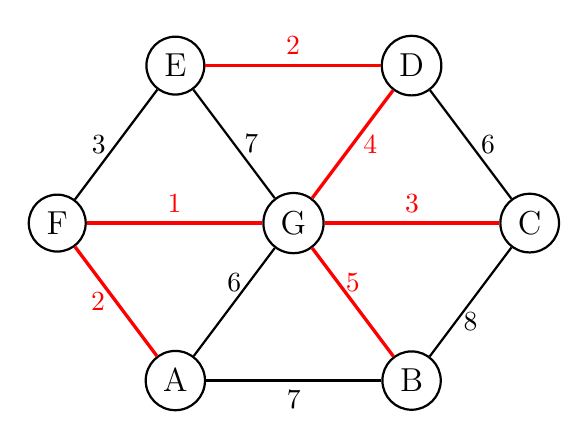
\begin{tikzpicture}
        [node/.style={circle,draw,minimum size=2em, thick, font=\large},
        edge/.style={thick},
        mst/.style={very thick, red}]
        
        % Vertices in a circular arrangement
        \node[node] (A) at (0,0) {A};
        \node[node] (B) at (3,0) {B};
        \node[node] (C) at (4.5,2) {C};
        \node[node] (D) at (3,4) {D};
        \node[node] (E) at (0,4) {E};
        \node[node] (F) at (-1.5,2) {F};
        \node[node] (G) at (1.5,2) {G};
        
        % Non-MST edges (normal black edges)
        \draw[edge] (A) -- (B) node[midway, below] {7};
        \draw[edge] (B) -- (C) node[midway, below] {8};
        \draw[edge] (C) -- (D) node[midway, right] {6};
        \draw[edge] (A) -- (G) node[midway, above] {6};
        \draw[edge] (E) -- (G) node[midway, right] {7};
        \draw[edge] (F) -- (E) node[midway, left] {3};
        
        % MST edges (highlighted in red)
        \draw[mst] (A) -- (F) node[midway, left] {2};
        \draw[mst] (G) -- (D) node[midway, right] {4};
        \draw[mst] (F) -- (G) node[midway, above] {1};
        \draw[mst] (G) -- (C) node[midway, above] {3};
        \draw[mst] (E) -- (D) node[midway, above] {2};
        \draw[mst] (B) -- (G) node[midway, above] {5};
        
    \end{tikzpicture}
    \caption{Um grafo não-direcionado com 7 vértices. As arestas em vermelho formam uma árvore geradora mínima (MST) de peso total 17.}
    \label{fig:mst_example}
\end{figure}

Existem diversas famílias de grafos, de modo que cada uma é adequada para resolver um tipo de problema particular. Iremos tratar inicialmente do \textbf{problema de conexidade em grafos dinâmicos}, que consiste em manter um grafo dinâmico que sofre uma sequência de inserções e remoções de arestas. Entre essas modificações, realizamos consultas para verificar se dois vértices \textit{u} e \textit{v} estão conectados por algum caminho. Para este problema, iremos usar as \textbf{florestas} (coleção de árvores) como base para a construção do algoritmo.

Inicialmente, utilizaremos o \textbf{problema de conexidade em florestas dinâmicas} como base para construir o algoritmo do \textbf{problema de conexidade em grafos dinâmicos}, e, a partir este, construir o \textbf{algoritmo decremental para árvores geradoras de custo mínimo}. Tais problemas possuem soluções propostas por \textit{Holm, de Lichtenberg e Thorup} \cite{jacob_holm}, nas quais a nossa implementação será baseada, e usaremos \textit{C++} como linguagem do código, onde disponibilizamos no repositório do \textit{GitHub} \cite{chung2025}.

\pagestyle{mainmatter}
%!TeX root=../tese.tex
%("dica" para o editor de texto: este arquivo é parte de um documento maior)
% para saber mais: https://tex.stackexchange.com/q/78101

\chapter{Conexidade em florestas dinâmicas}

\section{Definição}

Rodrigues \cite{arthur}, em sua dissertação do mestrado, estudou, entre outros assuntos, o problema da conexidade em florestas dinâmicas e implementou o seu algoritmo, que foi proposto na Seção 2 do artigo de Holm, de Lichtenberg e Thorup \cite{jacob_holm}. No Capítulo 2 da sua dissertação ele descreve as rotinas principais do algoritmo, baseado em \textit{Euler tour trees}, e realiza uma análise minuciosa da complexidade de tempo das funções dos pseudocódigos. Dada essas circunstâncias, optamos por não apresentar uma descrição detalhada desse algoritmo, explicando brevemente sobre o que as rotinas principais fazem, bem como algumas diferenças da nossa implementação em código comparadas com a de Rodrigues.  

O problema da conexidade em florestas dinâmicas pode ser considerada uma simplificação do problema de conexidade em grafos dinâmicos, quando o grafo em questão é uma floresta. A biblioteca que usaremos contém os seguintes métodos:

\begin{itemize}
    \item \texttt{\textbf{florestaDinâmica(F, n)}}: devolve uma floresta dinâmica $F$ com $n$ vértices isolados;
    \item \texttt{\textbf{conectado(F, u, v)}}: devolve verdadeiro se \textit{u} e \textit{v} estão na mesma componente da floresta $F$ e falso caso contrário;
    \item \texttt{\textbf{ligue(F, u, v)}}: insere uma aresta \textit{uv} na floresta $F$;
    \item \texttt{\textbf{corte(u, v)}}: remove a aresta \textit{uv} da floresta $F$;
\end{itemize}

Utilizamos árvores \textit{splay}, que foram desenvolvidas por \textit{Sleator e Tarjan} \cite{sleator}. Árvores \textit{splay} são árvores binárias de busca (ABBs) que possuem uma rotina extra (além das usuais de busca, inserção e remoção) chamada \textit{splay}, que é acionada ao final de cada operação feita na árvore, de modo que é sempre aplicada ao nó mais profundo visitado. Assim, a árvore fica mais balanceada à medida que a acionamos mais devido às rotações que acontecem na árvore. Isso faz com que o custo amortizado da operação \textit{splay} seja $O(\lg n)$, e que também uma sequência de $m$ acessos em uma árvore \textit{splay} tenha custo amortizado $O(m \lg n)$.  Como também já existe bastante literatura sobre árvores \textit{splay}, então assumiremos a corretude desta estrutura de dados.  

As árvores da floresta guardam as trilhas eulerianas dos vértices, em inglês \textit{Euler Tour Trees}, que foram propostas por \textit{Tarjan e Vishkin} \cite{tarjan} em 1985, de modo que cada trilha representa uma árvore. O nome da técnica de construção da árvore a partir da trilha se chama \textit{Euler tour technique}, que é descrita no capítulo 2.1 da dissertação de \textit{Rodrigues} \cite{arthur}.   

%!TeX root=../tese.tex
%("dica" para o editor de texto: este arquivo é parte de um documento maior)
% para saber mais: https://tex.stackexchange.com/q/78101

\chapter{Algoritmo para MSF decremental}

\enlargethispage{.8\baselineskip}

Neste capítulo, estudaremos o problema da árvore geradora mínima em grafos dinâmicos. 
Dado um grafo conexo $G$ com um custo associado a cada uma de suas arestas, 
o problema da árvore geradora mínima consiste em determinar uma árvore geradora
de G com custo mínimo, onde o custo de uma árvore é a soma dos custos de suas arestas. 
Como estamos interessados em grafos dinâmicos, é natural remover a restrição de que o 
grafo seja conexo, e neste caso considerar florestas geradoras maximais de custo mínimo 
(MSF, do inglês \emph{minimum spanning forest}). Chamamos um grafo com um custo 
associado a cada aresta de \textbf{grafo ponderado}. 

O problema da árvore geradora mínima em grafos ponderados (conexos) estáticos pode ser 
resolvido eficientemente, por exemplo, pelos algoritmos de Kruskal e de Prim. O algoritmo de Kruskal 
utiliza uma estrutura de dados clássica conhecida como union-find, enquanto que o algoritmo
de Prim utiliza uma fila de prioridades. Não há na literatura uma versão destes algoritmos 
para grafos dinâmicos. Isso talvez se deva à característica essencialmente sequencial destes
algoritmos, que modificam suas estruturas internas conduzidos por uma ordem de eventos.
Uma alteração no grafo poderia levar a uma alteração em toda a sequência de eventos 
nesses algoritmos a partir de um certo ponto, e com isso não há uma versão eficiente deles
que acomode alterações no grafo. 

Por outro lado, Holm, de Lichtenberg e Thorup~\cite{jacob_holm} propuseram uma adaptação do seu algoritmo para conexidade em 
grafos dinâmicos, apresentado no Capítulo 2, para que este mantenha, de maneira eficiente, 
uma floresta geradora maximal de custo mínimo em um grafo ponderado que pode sofrer 
remoções de arestas.  Ou seja, eles propuseram um algoritmo que resolve de maneira 
eficiente o problema que chamamos de MSF decremental.  Neste capítulo, descreveremos
esse algoritmo, descrevendo a adaptação do algoritmo descrito no Capítulo 2 para que este 
passe a resolver o problema da MSF decremental.  

\section{Biblioteca da MSF decremental}
\label{sec:decremental-msf-library}

Implementar o algoritmo decremental para florestas geradoras maximais de custo mínimo (MSF, de \textit{Minimum Spanning Forest}) resume-se à construção da seguinte biblioteca de forma eficiente:

\begin{itemize}
    \item \texttt{\textbf{MSFDecremental(n, E)}}: contrói e devolve um grafo ponderado $G$ com $n$ vértices e as arestas $E$;
    \item \texttt{\textbf{conectadosMSF(G, u, v)}}: devolve verdadeiro se os vértices $u$ e $v$ estão na mesma componente de $G$ e falso caso contrário;
    \item \texttt{\textbf{removaMSF(G, u, v)}}: remove a aresta $uv$ do grafo $G$.
\end{itemize} 

Note que, diferente da biblioteca do algoritmo de conexidade em grafos dinâmicos, apresentada na Seção~\ref{sec:dynamic-graph-routines}, na MSF decremental não temos um método equivalente a \texttt{adicioneGD} disponível para o usuário. Em nossa implementação \cite{chung2025}, para criarmos um grafo $G$ de $n$ vértices e $m$ arestas ponderadas dadas no conjunto $E$, chamamos \texttt{MSFDecremental($n$, $E$)}, onde inserimos $n$ vértices isolados e, em seguida, ordenamos e inserimos essas $m$ arestas em ordem crescente de peso, usando uma biblioteca pronta do $\emph{C++}$, que consome tempo esperado $\Oh(n \lg n)$. Estas $m$ arestas são inseridas uma a uma acionando \texttt{adicioneMSF(u, v, w)}, onde $u$ e $v$ são pontas da aresta e $w$ é o peso dela.

A rotina \texttt{adicioneMSF} é acionada somente dentro do construtor. Por ser uma rotina privada, ou seja, não está disponível para o usuário, após a inserção destas arestas, não é permitido mais operações de inserção, somente de remoção de arestas. Para o usuário, então, só estarão disponíveis as rotinas \texttt{conectadosMSF} e \texttt{removaMSF} como consultas ao grafo. A versão totalmente dinâmica, que inclui a rotina \texttt{adicioneMSF} para o usuário, será estudada posteriormente na Seção~\ref{sec:fully-MSF}.

O construtor \texttt{MSFDecremental}, devido à ordenação de arestas, possui consumo de tempo $\Oh(n \lg n)$. Já a rotina \texttt{conectadosMSF} possui consumo de tempo amortizado $\Oh(\lg n)$, a mesma do \texttt{conectadosGD}. Como estes dois métodos são muito parecidos com os do algoritmo de conexidade em grafos dinâmicos, passaremos brevemente sobre eles, e detalharemos mais a rotina \texttt{removaMSF}, que possui a rotina auxiliar \texttt{substituaArestaMSF} implementada de maneira diferente do \texttt{substituaAresta} do algoritmo de conexidade em grafos dinâmicos. 

Usaremos várias definições já apresentadas no algoritmo do grafo dinâmico, incluindo as mesmas invariantes apresentadas na Seção~\ref{sec:level-slicing}, os mesmos tipos de arestas da Seção~\ref{sec:dynamic-graph-edge-types} e nós das florestas apresentados na Seção~\ref{sec:graph-nodes}. A seguir, apresentaremos as rotinas da MSF decremental e alguns ajustes a serem feitos. 

\subsection{Listas de adjacências}
\label{sec:adjancency-lists-min-heap}

Na Seção~\ref{sec:dynamic-graph-edge-types}, apresentamos a biblioteca de \texttt{listasDeAdjacências}, onde usamos um mapa hash para inserir ou remover um vértice $v$ da lista de $u$, além de percorrer os vizinhos da lista de $u$. No algoritmo da MSF decremental, quando removemos uma aresta de nível $i$ da floresta $F_i$, uma componente desta será quebrada em duas, $T_u$ e $T_v$, da mesma forma que no algoritmo de conexidade em grafos dinâmicos. A diferença é que, no caso da MSF decremental, precisamos buscar por uma aresta substituta que tenha o menor peso e que ligue $T_u$ a~$T_v$. Não podemos simplesmente percorrer todos os vizinhos $v$ de cada vértice $u$ em $T_u$, verificar se $uv$ reconecta as componentes separadas e se é de menor peso dentre todas as substitutas, já que isso seria ineficiente.

Assim, fica claro que seria bom percorrer as arestas reservas em ordem crescente de peso e testar se alguma é substituta nesta ordem. Por isso, em vez de usar um mapa hash para mapear os vizinhos das listas de adjacências de cada vértice, usaremos um min-heap. Na verdade, como estamos trabalhando com nós de vértice e de aresta, cada nó de vértice $u$ guardará um min-heap com os vizinhos de $u$, onde a chave dessa estrutura de dados para um vizinho $v$ será o peso da aresta $uv$. Nós de aresta também guardarão um min-heap, porém vazio. 

A biblioteca do min-heap está descrita a seguir.

\begin{itemize}
    \item \texttt{\textbf{MinHeap(u)}}: cria um min-heap vazio para o vértice $u$ (em nossa implementação, criamos um vetor vazio);
    \item \texttt{\textbf{éVazio(MH, u)}}: devolve verdadeiro se o min-heap MH de $u$ está vazio e falso caso contrário;
    \item \texttt{\textbf{tamanho(MH, u)}}: retorna a quantidade de vizinhos no min-heap MH de $u$;
    \item \texttt{\textbf{remova(MH, u, v)}}: remove o vizinho $v$ do min-heap MH de $u$;
    \item \texttt{\textbf{consulteMínimo(MH, u)}}: retorna um par $\{v, p\}$ do min-heap MH de $u$, onde $v$ é um vizinho de $u$ com chave mínima $p$;
    \item \texttt{\textbf{extraiaMínimo(MH, u)}}: remove o par $\{v, p\}$ do min-heap MH de $u$, onde $v$ é o vizinho de $u$ com chave mínima $p$;
    \item \texttt{\textbf{insira(MH, u, v, p)}}: insere o vizinho $v$ no min-heap MH de $u$, onde $p$ é sua chave, ou seja, é o peso da aresta $uv$.
\end{itemize} 

Os métodos \texttt{remova}, \texttt{extraiaMínimo} e \texttt{insira} consomem tempo O($\lg n)$ usando uma implementação tradicional de heap sort de Thomas H. Cormen et al. \cite{clrs}. O resto dos métodos consomem tempo constante, e eles serão necessários para buscar a aresta substituta de peso mínimo, como descreveremos mais à frente.

Com base na biblioteca do min-heap, podemos definir a biblioteca das listas de adjacências da MSF decremental. 

\begin{itemize}
    \item \texttt{\textbf{listasDeAdjacênciasMSF(n)}}: constrói e devolve um grafo com $n$ vértices e sem arestas, representado por listas de adjacências;
    \item \texttt{\textbf{adicioneLAMSF(R, u, v, p)}}: adiciona o vértice $u$ na lista de adjacências de $v$ em $R$ e vice-versa, considerando que o peso de $uv$ é $p$;
    \item \texttt{\textbf{removaLAMSF(R, u, v)}}: remove o vértice $u$ da lista de adjacências de $v$ em $R$ e vice-versa.
\end{itemize} 

Uma chamada à rotina \texttt{adicioneLAMSF(R, u, v, p)} aciona \texttt{insira(MH, u, v, p)} e \texttt{insira(MH, v, u, p)}, consumindo tempo $\Oh(\lg n)$. Similarmente, uma chamada à rotina \texttt{removaLAMSF(R, u, v)} aciona \texttt{remova(MH, u, v)} e \texttt{remova(MH, v, u)}, consumindo também tempo $\Oh(\lg n)$.

Como o min-heap é uma estrutura de dados bastante conhecida, não iremos descrever a sua implementação em detalhes. O objetivo é ressaltar as diferenças entre as listas de adjacências utilizadas no algoritmo de conexidade em grafos dinâmicos e na MSF decremental, e como essa mudança afetará o comportamento do método \texttt{substituaArestaMSF} da MSF decremental.

\section{Rotinas da biblioteca da MSF decremental}

\subsection{Criação do grafo}

A rotina \texttt{MSFDecremental}, como se pode ver no Programa~\ref{prog:newDecrementalMSF}, é bem parecida com a do grafo dinâmico, descrita na Seção~\ref{sec:dynamic-graph-creation}. 

\begin{programruledcaption}{\texttt{MSFDecremental($n$, $E$)} \label{prog:newDecrementalMSF}}
    \noindent\textbf{Entrada}: Recebe o número $n$ de vértices do grafo e um conjunto de arestas $E$. \\
    \textbf{Saída}: Devolve um grafo $G$ com $n$ vértices e $m$ arestas ponderadas.
    \vspace{-0.5\baselineskip}
    \begin{lstlisting}[
        language={[brazilian]pseudocode},
        style=pseudocode,
        style=wider,
        functions={},
        specialidentifiers={},
        escapeinside={(*@}{@*)},
    ]
    L := $\left\lceil \lg n \right\rceil$
    $\dotvar{G}{nívelMax}$ := L
    \textbf{para} $i$ := $1$ \textbf{até} $L$ \textbf{faça}
        $G.F_i$ := \texttt{florestaDinâmica($n$)}
        $G.R_i$ := \texttt{listasDeAdjacênciasMinHeap($n$)}
    $\dotvar{G}{nível}$ := \texttt{novoMapaHash($n$)}
    \texttt{ordene($E$)} (*@\hfill $\triangleright$ ordena as arestas do conjunto $E$ em ordem crescente@*)
    \textbf{para cada aresta} ($u$, $v$, $p$) \textbf{em} $E$ \textbf{faça}
        \texttt{adicioneMSF}($G$, $u$, $v$, $p$)
    \textbf{retorne} G
    \end{lstlisting}
    \vspace{-0.5\baselineskip}
\end{programruledcaption}

Podemos notar algumas diferenças quando comparamos o construtor \texttt{MSFDecremental} com o \texttt{grafoDinâmico}. Na MSF decremental, além de inicializarmos $\left\lceil \lg n \right\rceil$ listas de adjacências e $\left\lceil \lg n \right\rceil$ florestas dinâmicas, ordenamos arestas do conjunto $E$ em ordem crescente e inserimos uma a uma chamando \texttt{adicioneMSF}, que está descrito abaixo.

\begin{programruledcaption}{\texttt{adicioneMSF($G$, $u$, $v$, $p$)} \label{prog:addMSF}}
    \noindent\textbf{Entrada}: Recebe dois vértices $u$ e $v$ do grafo $G$, com $u < v$, e o peso $p$ da aresta $uv$. \\
    \textbf{Efeito}: Adiciona a aresta $uv$ de peso $p$ no grafo $G$.
    \vspace{-0.5\baselineskip}
    \begin{lstlisting}[
        language={[brazilian]pseudocode},
        style=pseudocode,
        style=wider,
        functions={},
        specialidentifiers={},
        escapeinside={(*@}{@*)},
    ]
    L := $\dotvar{G}{nívelMax}$
    $\dotvarm{G}{nível}{u,v}$ := $L$
    \textbf{se} \texttt{conectadosFD($G.F_{L}$, $u$, $v$)} \textbf{então} (*@\hfill $\triangleright$ $uv$ é aresta reserva@*)
        \texttt{adicioneLAMSF($G.R_{L}$, $u$, $v$, $p$)}
        \texttt{incrementeArestasReservasDeNível($G.F_{L}$, $G.R_{L}$, $u$)}
        \texttt{incrementeArestasReservasDeNível($G.F_{L}$, $G.R_{L}$, $v$)}
    \textbf{senão}
        \texttt{adicioneFD($G.F_L$, $u$, $v$, $p$)}
        \texttt{atualizeÉNível($G.F_L$, $u$, $v$, $\textbf{verdadeiro}$)}
    \end{lstlisting}
    \vspace{-0.5\baselineskip}
\end{programruledcaption}

Como mencionado antes, a rotina \texttt{adicioneMSF} é acionada exclusivamente em \texttt{MSFDecremental}. Além disso, a única diferença entre a \texttt{adicioneMSF} e a \texttt{adicioneGD} que vimos é que, na primeira, estamos guardando o peso das arestas quando as inserimos no grafo. Portanto, ambas consomem o mesmo tempo amortizado $\Oh(\lg n)$ e as três invariantes são preservadas ao acionar \texttt{adicioneMSF}, já que estamos sempre inserindo arestas com nível $\left\lceil \lg n \right\rceil$ em $F_L$ e as florestas de níveis inferiores não são afetadas com a inserção.

\subsection{Consultas de conexidade na MSF decremental}
\label{sec:connectivity-test-MSF}

O método \texttt{conectadosMSF}, que está descrito abaixo, é igual ao \texttt{conectadosGD}. Mudamos somente o nome para ficar coerente com os nomes dos métodos da biblioteca da MSF decremental. 

\begin{programruledcaption}{\texttt{conectadosMSF($G$, $u$, $v$)} \label{prog:connectedMSF}}
    \noindent\textbf{Entrada}: Recebe dois vértices $u$ e $v$ do grafo $G$. \\
    \textbf{Saída}: Devolve um booleano indicando se $u$ e $v$ estão conectados em $G$.
    \vspace{-0.5\baselineskip}
    \begin{lstlisting}[
        language={[brazilian]pseudocode},
        style=pseudocode,
        style=wider,
        functions={},
        specialidentifiers={},
        escapeinside={(*@}{@*)},
    ]
    L := $\dotvar{G}{nívelMax}$
    retorne \texttt{conectadosFD($G.F_L$, $u$, $v$)}
    \end{lstlisting}
    \vspace{-0.5\baselineskip}
\end{programruledcaption}

\raggedbottom

Da mesma forma que em \texttt{conectadosGD}, a rotina \texttt{conectadosMSF} também consome tempo amortizado $\Oh(\lg n)$. Além disso, a rotina de consulta não altera o nosso grafo, incluindo florestas e listas de adjacências, já que não há nenhuma modificação neles. Isso implica que as três invariantes são mantidas. 


%!TeX root=../tese.tex
%("dica" para o editor de texto: este arquivo é parte de um documento maior)
% para saber mais: https://tex.stackexchange.com/q/78101

\chapter{Algoritmo totalmente dinâmico para MSF}

\section{Definição}
\label{sec:fully-MSF}


%%%%%%%%%%%%%%% SEÇÕES FINAIS (BIBLIOGRAFIA E ÍNDICE REMISSIVO) %%%%%%%%%%%%%%%%

% O comando backmatter desabilita a numeração de capítulos.
\backmatter

\pagestyle{backmatter}

% Espaço adicional no sumário antes das referências / índice remissivo
%\addtocontents{toc}{\vspace{2\baselineskip plus .5\baselineskip minus .5\baselineskip}}

% A bibliografia é obrigatória

\printbibliography[
  %title=\refname\label{sec:bib}, % "Referências", recomendado pela ABNT
  title=\bibname\label{sec:bib}, % "Bibliografia"
  heading=bibintoc, % Inclui a bibliografia no sumário
]

%\printindex % imprime o índice remissivo no documento (opcional)

\end{document}
